\subsection{Find Chest XRay(s) Orientation}
\label{sec:warmup2}

    In this introductory warmup exercise, chest X-rays were provided, and the task involved training/fine-tuning a model to determine the orientation of these X-rays.

\subsubsection{Dataset}
    The provided dataset consists of Grayscale X-ray images with 948 training samples depicting various orientations and an additional 40 samples for testing. All images are of size $128 \times 128$ and are oriented either as up (0), right (1), down (2), or left (4). Due to the absence of a dedicated validation set in the given dataset, I have randomly partitioned the training samples into training and validation sets in 9:1 ratio. 
\subsubsection{Model Used}

    For this task, I utilized ResNet18 as the backbone model with pre-trained weights from ImageNet. Since ResNet18 was originally trained on ImageNet, its output tensor has a size of (n, 1000). However, in the given problem, we are specifically dealing with 4 classes (up, right, down, left). Therefore, I introduced few fully connected layer followed by a sigmoid layer for each class. \Cref{fig:orientation_model} shows the graphical representation of the used model architecture.
    
    % \begin{figure}[htbp]
    %     \centering
    %     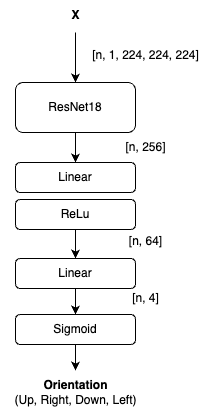
\includegraphics[width=0.4\linewidth]{images/OrientationModel.png}
    %     \caption{Graph of model used}
    %     \label{fig:model_graph}
    % \end{figure}

\subsubsection{Training}
    
    The model is trained using the Bbinary cross-entropy loss with adam as the optimizer. The model was trained for with learning rate ot $10^{-4}$ for $5$ epochs. \Cref{fig:orientation-learning-curve} shows the learning curve and it can be infered from this that the model is neither overfitted, nor underfitted.

    \begin{figure}[htbp]
        \centering
        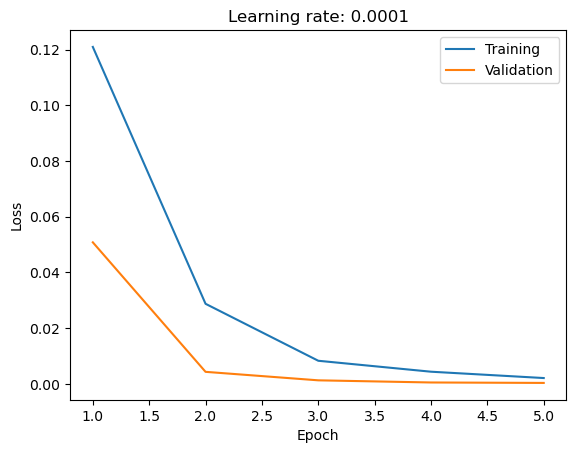
\includegraphics[width=\linewidth]{../plots/orientation/learning-0.0001-adam.png}
        \caption{Learning curve of model trained for classifying the orientation of the chest xray.}
        \label{fig:orientation-learning-curve}
    \end{figure}

\subsubsection{Results}

    \begin{figure*}[!htbp]
        \centering
        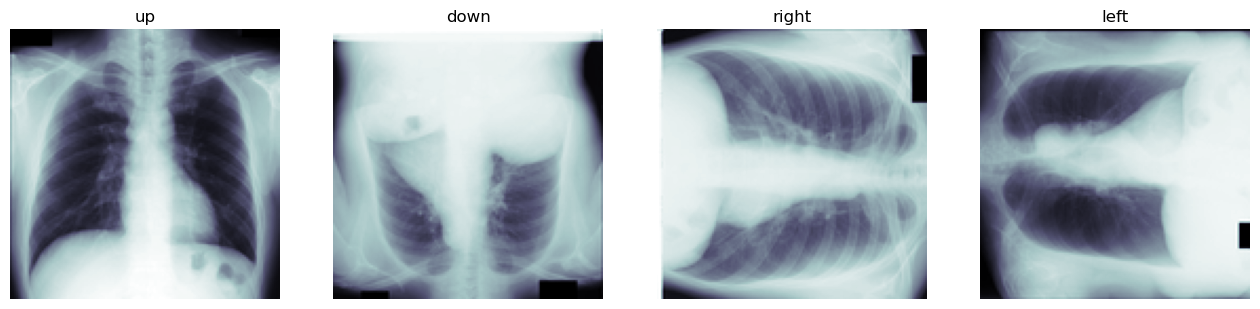
\includegraphics[width=\linewidth]{../plots/orientation/result.png}
        \caption{Predictions of few test samples to find orientation of chest xray}
        \label{fig:orientation-results}
    \end{figure*} 

    After fine-tuning the model with the ResNet18 backbone, the model was transitioned to testing and evaluated on the provided test samples. The accuracy and AUC of the model is reported in \cref{tab:classification-model-results}. \Cref{fig:orientation-results} showcases some of the test samples along with model predection.
